\documentclass[a4paper, 12pt]{article}

\usepackage{../../../LaTeX_packages/TP_style}

\begin{document} % ----------------------------------------------------------- %


\input{../../../LaTeX_packages/TP_header_L3_MIAGE.tex}

% TITLE
% -----
\tptitle{2}{How data structures affect models}

% BODY
% ----
The goal of this practical is to learn how to implement various python data structures (such as lists,sets and dictionary) in PULP models. 

\section{An illustration with the admissible cells problem}

\paragraph{} Given a rectangular grid \(T^{m \times n}\) of boxes called \emph{cells}. Some of these cells are \emph{admissible}, the others are \emph{non-admissible}. Also are given \(m+n\) non-negative integers \(l_0 \ldots l_{m-1}\), \(c_0 \ldots c_{n-1}\). The goal is to fill in the admissible cells with positive integers such as:

\begin{itemize}[label=---]\itemsep=0em
  \item The sum of the numbers allocated on the admissible cells on row \(i\) should be less or equal than \(l_i\);
  \item The sum of the numbers allocated on the admissible cells on column \(j\) should be less or equal than \(c_j\);
  \item The total sum of all these numbers should be maximum.
\end{itemize}

\phantom{}

\noindent \textbf{Example:} Let:
\begin{align*}
  (m & = 4) & l_0 & =9 & l_1 & =10 & l_2 & =15 & l_3 & =2 &     &    \\
  (n & = 5) & c_0 & =7 & c_1 & =5  & c_2 & =9  & c_3 & =4 & c_4 & =8
\end{align*}

\indent and the set of admissible cells is:
\[
  A=\{(0,0),\, (0,1),\, (1,0),\, (1,2),\, (1,3),\, (2,1),\, (2,4),\, (3,2),\, (3,4)\}
\]
\indent where the first index corresponds to the row, second index to the column number.

\begin{figure}[H]
  \begin{center}
    \begin{minipage}{0.5\textwidth}
      \centering
      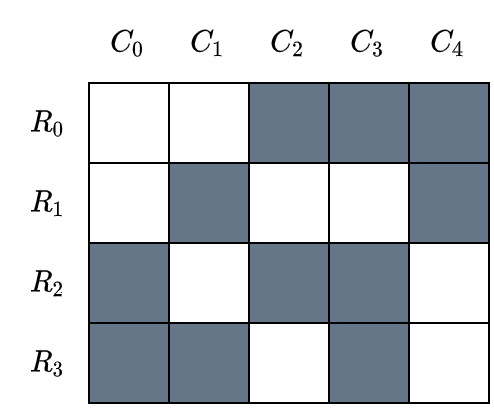
\includegraphics[width=\textwidth]{./img/admissible_cells.png}
    \end{minipage}
    \hfill
    \begin{minipage}{0.48\textwidth}
      \centering
      \caption{Only the blank cells can be filled with a value. \(l_i\) is the limit value of the sum of cells in row \(i\), \(c_j\) is the limit value of the sum of cells in column \(j\)}\label{fig:admissible_cells}
    \end{minipage}
  \end{center}
\end{figure}


\section{Understanding and extending models using different data structures}
The \texttt{TP2} folder contains four python files : 
\begin{enumerate}
  \item \texttt{tp2\_admissible\_cells\_array\_partial\_correction.py}, 
  \item  \texttt{tp2\_admissible\_cells\_set\_partial\_correction.py}, 
  \item \texttt{tp2\_setting\_input\_data.py} 
  \item  \texttt{tp2\_read\_data\_files.py}. 
\end{enumerate}
The first two programs propose two different approaches for implementing the admissible cells problem. The first code uses data structure \texttt{list}, while the second one uses data structures \texttt{set} and  \texttt{dictionary}.  These programs are incomplete, some constraints are missing. 

\begin{question}
  Your first task is to read and understand them.
  Run them with: 
\begin{minted}[bgcolor=LightGray]{bash}
(.venv_3) python3 tp2_admissible_cells_array_partial_correction.py 
\end{minted}

\begin{minted}[bgcolor=LightGray]{bash}
(.venv_3) python3 tp2_admissible_cells_set_partial_correction.py 
\end{minted}
    
\noindent What is the solution?
\end{question}
\begin{question}
  What are the missing constraints? Add them and run the programs again. Explain the changes made to the calculated solutions as a result of adding new constraints.  
\end{question}

\begin{question} 
  Figures \ref{fig:posdiagonal} and \ref{fig:negdiagonal} illustrate the two types of diagonal of a matrix (the positive diagonal \ref{fig:posdiagonal} and the negative diagonal \ref{fig:negdiagonal}). 

  \begin{enumerate}
    \item  Give the linear constraints that model any of the above requirements. 
    \item Choose one the previously described data structure and add these constraints in your PULP program. 
  \end{enumerate}


\end{question}

\begin{figure}[H]
  \begin{center}
    \begin{minipage}{0.5\textwidth}
      \centering
      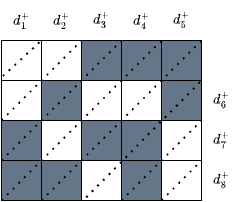
\includegraphics[width=0.7\textwidth]{./img/pos_diagonal_adm_cells.png}
      \caption{The sum of the numbers allocated on the admissible cells on the positive diagonal \(i\) should be less or equal than the given number \(d^+_i\);}\label{fig:posdiagonal}
    \end{minipage}
    \hfill
    \begin{minipage}{0.48\textwidth}
      \centering
      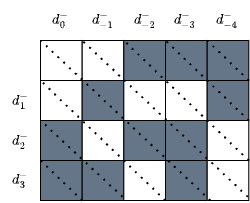
\includegraphics[width=0.7\textwidth]{./img/neg_diagonal_adm_cells.png}
      \caption{The sum of the numbers allocated on the admissible cells on the negative diagonal \(i\) should be less or equal than the given number \(d^-_i\)}\label{fig:negdiagonal}
    \end{minipage}
  \end{center}
\end{figure}


The last two codes contain functions for entering input data for eligible cells. 
The file 
 \texttt{tp2\_setting\_input\_data.py} describes the function \texttt{get\_adm\_cells\_data\_bis} which is used to enter input data in the same way as in TP1. This is the function that is used by default in the above programs. 


 The file \texttt{tp2\_read\_data\_files.py}  is a  FileReader API. It codes functions to extract admissible cells from files in \texttt{data} directory, and a function to parse command line's argument. It is not necessary to understand how they work, you need only to use them.

Especially, the function \texttt{get\_adm\_cells\_data} lets you iterating over it to get admissible cells data from each file. You can use it as following:

\begin{minted}[bgcolor=LightGray]{python}
for adm_cells, row_limits, col_limits in get_adm_cells_data():
    # adm_cells: list of tuple (row_i, col_j)
    #   corresponding to admissible cells
    # row_limits: list of row limits (int)
    # col_limits: list of column limits (int)
    solve_admissible_cells(adm_cells, row_limits, col_limits)
\end{minted}

In fact, \texttt{get\_adm\_cells\_data} \emph{yield} the three lists instead of returning them. It allows to iterate over the function in a stream way.

\begin{question}
Find how and where these functions can be used in the above codes.  Make the necessary in order to use them. 
Run them with:
\begin{minted}[bgcolor=LightGray]{bash}
(.venv_3) python3  tp2_admissible_cells_array_partial_correction.py
\end{minted}
  and 
\begin{minted}[bgcolor=LightGray]{bash}
(.venv_3) python3  tp2_admissible_cells_set_partial_correction.py 
\end{minted} 

\noindent What is the solution?
\end{question}


\begin{question}
  In order to test more complex instances, you can run your program like this:
\begin{minted}[bgcolor=LightGray]{bash}
(.venv_3) python3 your_prog.py --all-data > tp2_all_results.log
\end{minted}
 
  Run the program for all the data and plot the CPU time according to the number of variables, and according to the number of constraints, with the method of your choice.

  \phantom{}

  \noindent\textbf{Tip:} you can use \texttt{CTRL+F} on \texttt{tp2\_all\_results.log} and search for \texttt{FILE} word in order to find very quickly statistics.
\end{question}

\end{document} % ------------------------------------------------------------- %
